


\documentclass[12pt]{article}


\usepackage{scicite}
\usepackage{fixltx2e}
\usepackage{mathtools}
\usepackage{graphicx}



\usepackage{times}



\topmargin 0.0cm
\oddsidemargin 0.2cm
\textwidth 16cm 
\textheight 21cm
\footskip 1.0cm

\renewcommand{\baselinestretch}{0.5} 


\newenvironment{sciabstract}{%
\begin{quote} \bf}
{\end{quote}}



\renewcommand\refname{References and Notes}


\newcounter{lastnote}
\newenvironment{scilastnote}{%
\setcounter{lastnote}{\value{enumiv}}%
\addtocounter{lastnote}{+1}%
\begin{list}%
{\arabic{lastnote}.}
{\setlength{\leftmargin}{.22in}}
{\setlength{\labelsep}{.5em}}}
{\end{list}}




\title{{\it \textbf{Experiment 1:\hspace{0.5cm} Transfer Characteristics of a CS Amplifier}\/} } 




\author
{Satyanand 14EC10049\\
\normalize{Rohit Kumar 14EC10043}
}


% \date{}






\begin{document} 

% Double-space the manuscript.

%spacing between lines
% \begin{center}
%       \Large\textbfExperiment 1:\hspace{0.5cm} D.C. characterization and finding parameters of transistors}\\
%       \large\textit{Satyanand 14EC10049\\
%       \normalize{Rohit Kumar 14EC10043}
%    \end{center}
\baselineskip14pt

% Make the title.

\maketitle 








\renewcommand{\baselinestretch}{0.5} 

\section*{Objective}
%\vspace{-\baselineskip}
\begin{itemize}
\item To obtain the transfer characteristics of a NMOS CS amplifier when (i) RD =2.43 k$\Omega$, (ii) RD = 4.58 k$\Omega$ and (iii) Coupled NMOS with RD = 4.58 k$\Omega$.
\item To plot the derivative (gain) in MATLAB and obtain the maximum gain and Vmax i.e. the input voltage VIN at which the maximum gain occurs.
\item To use the techniques of polynomial fitting and fast fourier transform to find the frequency spectrum of amplitude of Vout and thus determine the Total Harmonic Distortion (THD).
\item To check the THD value for a given input signal when we cascade multiple amplifier stages together. Also, to see whether we get any difference in THD in case we change the order of the amplifiers (high gain first vs low gain first).
\item To check the THD degradation as the output bias point is skewed away from the mid value of VDD/2.
\item To check the THD value for increasing signal magnitude and different gain values.
\end{itemize}


\section*{Components}
\begin{itemize}
    \item MOSFET
    \item Breadboard
    \item Resistors 
    \item Potentiometers
    \item Connecting wires
\end{itemize}

\section*{Circuit Diagram}
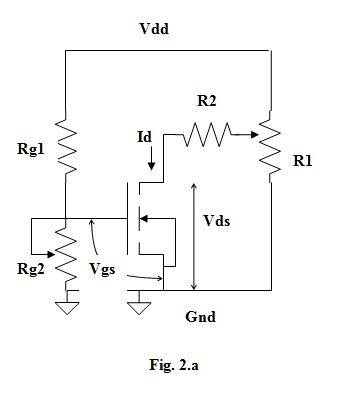
\includegraphics{ckt.jpg}
  \caption{Circuit diagram}
  %\label{fig:boat1}
  
%\section*{Design Steps:}

\section*{Observation Table}
\subsection{ V$_o_u_t$ vs V$_i_n$ for R$_D$=}
\begin{center}
 \begin{tabular}{|| c | c||} 
 \hline
 V$_o_u_t$(V) &  V$_i_n$(V)\\ [0.5ex] 
 \hline\hline
 1.53 & 12.02 \\
\hline
1.78 & 12.01 \\
\hline
1.97 & 11.83 \\
\hline
2.14 & 11.54 \\
\hline
2.24 & 11.29 \\
\hline
2.31 & 11.05 \\
\hline
2.36 & 10.88 \\
\hline
2.45 & 10.54 \\
\hline
2.55 & 10.13 \\
\hline
2.63 & 9.78 \\
\hline
2.7 & 9.38 \\
\hline
2.77 & 9.04 \\
\hline
2.81 & 8.86 \\
\hline
2.87 & 8.57 \\
\hline
2.91 & 8.19 \\
\hline
2.98 & 7.81 \\
\hline
3 & 7.67 \\
\hline
3.06 & 7.27 \\
\hline
3.11 & 6.98 \\
\hline
3.17 & 6.55 \\
\hline
3.22 & 6.14 \\
\hline
3.3 & 5.64 \\
\hline
3.4 & 4.99 \\
\hline
3.43 & 4.57 \\
\hline
3.51 & 4.11 \\
\hline
3.61 & 3.83 \\
\hline
3.59 & 3.46 \\
\hline
3.64 & 2.94 \\
\hline
3.69 & 2.6 \\
\hline
3.74 & 2.08 \\
\hline
3.78 & 1.7 \\
\hline
3.85 & 1.22 \\
\hline
3.94 & 0.99 \\
\hline
4.1 & 0.8 \\
\hline
4.88 & 0.54 \\
\hline
5.86 & 0.41 \\
\hline
6.3 & 0.38 \\
\hline


\end{tabular}
\end{center}

\subsection{V$_o_u_t$ vs V$_i_n$ for R$_D$=}
\begin{center}
 \begin{tabular}{|| c | c||} 
 \hline
 V$_o_u_t$(V) &  V$_i_n$(V)\\ [0.5ex] 
 \hline\hline
 0.0 & 12.06 \\
\hline
1.33 & 12.07 \\
\hline
1.74 & 12.06 \\
\hline
2.27 & 11.58 \\
\hline
2.31 & 11.4 \\
\hline
2.42 & 11.13 \\
\hline
2.54 & 10.86 \\
\hline
2.67 & 10.48 \\
\hline
2.83 & 9.95 \\
\hline
3.03 & 9.15 \\
\hline
3.19 & 8.5 \\
\hline
3.27 & 8.07 \\
\hline
3.45 & 7.39 \\
\hline
3.56 & 6.86 \\
\hline
3.68 & 6.18 \\
\hline
3.8 & 5.53 \\
\hline
3.81 & 5.37 \\
\hline
3.86 & 5.1 \\
\hline
3.94 & 4.78 \\
\hline
4.07 & 3.89 \\
\hline
4.11 & 3.63 \\
\hline
4.19 & 3.13 \\
\hline
4.29 & 2.48 \\
\hline
4.35 & 2.16 \\
\hline
4.57 & 1.29 \\
\hline
4.73 & 1.1 \\
\hline
4.93 & 0.96 \\
\hline
5.42 & 0.78 \\
\hline
5.69 & 0.72 \\
\hline
6.15 & 0.64 \\
\hline
7.63 & 0.5 \\
\hline
10.14 & 0.4 \\
\hline
11.2 & 0.36 \\
\hline

\end{tabular}
\end{center}

\subsection{V$_o_u_t$ vs V$_i_n$ for coupled FETs}
\begin{center}
 \begin{tabular}{|| c | c||} 
 \hline
 V$_o_u_t$(V) &  V$_i_n$(V)\\ [0.5ex] 
 \hline\hline
 1.74 & 12.04 \\
\hline
1.88 & 11.9 \\
\hline
2.0 & 11.63 \\
\hline
2.14 & 11.13 \\
\hline
2.23 & 10.69 \\
\hline
2.28 & 10.38 \\
\hline
2.37 & 9.79 \\
\hline
2.44 & 9.29 \\
\hline
2.51 & 8.71 \\
\hline
2.58 & 8.13 \\
\hline
2.61 & 7.87 \\
\hline
2.65 & 7.52 \\
\hline
2.68 & 7.18 \\
\hline
2.74 & 6.55 \\
\hline
2.78 & 6.17 \\
\hline
2.82 & 5.69 \\
\hline
2.86 & 5.27 \\
\hline
2.88 & 5.0 \\
\hline
2.91 & 4.68 \\
\hline
2.95 & 4.17 \\
\hline
2.98 & 3.78 \\
\hline
3.03 & 3.25 \\
\hline
3.08 & 2.52 \\
\hline
3.12 & 2.09 \\
\hline
3.36 & 0.58 \\
\hline
4.17 & 0.31 \\
\hline
4.45 & 0.28 \\
\hline
4.83 & 0.25 \\
\hline
5.61 & 0.2 \\
\hline

 


\end{tabular}
\end{center}
 
 
 

\section*{Plots}

\subsection*{Plot of V_o_u_t vs V_i_n}
\begin{center}
    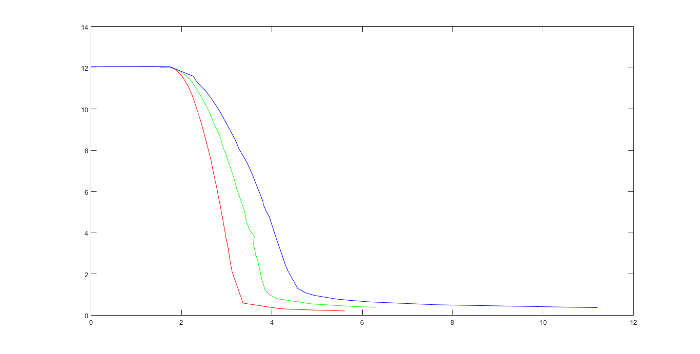
\includegraphics{data.png}
\end{center}

\subsection*{Gain versus V_i_n }
\begin{center}
    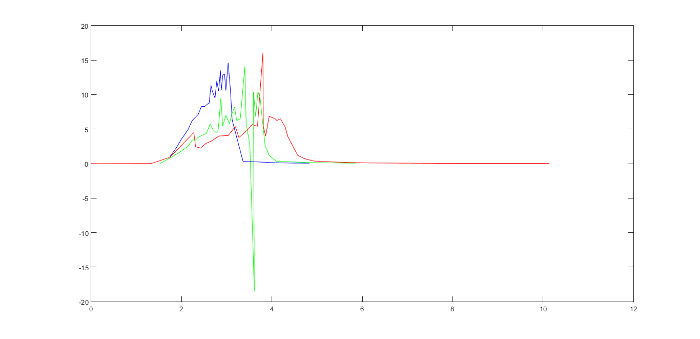
\includegraphics{gain_correct.png}
\end{center}

\subsection*{Gain versus V$_i_n$ with moving average }
Then, we take a moving average smoothing filter (included in the MATLAB library as a built-in function) to smoothen it. Given below are the unsmoothed and smoothed plots respectively.
\begin{center}
    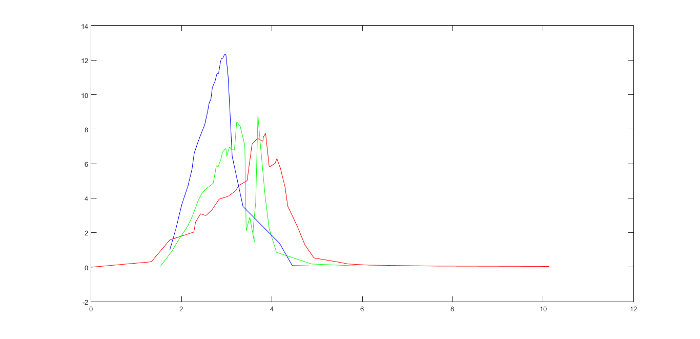
\includegraphics{gain_moving_avg.png}
\end{center}

\subsection*{Gain versus }
\begin{center}
    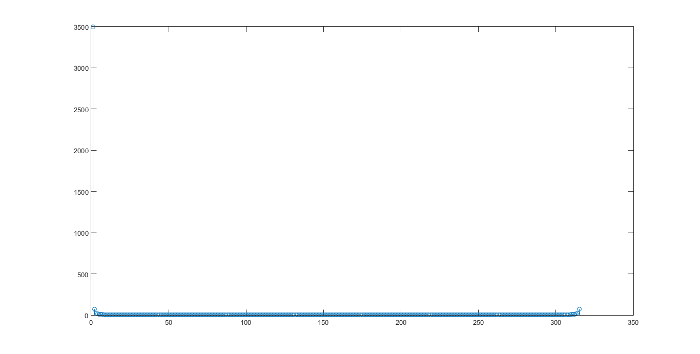
\includegraphics{stem1.png}
\end{center}

\subsection*{Gain versus }
\begin{center}
    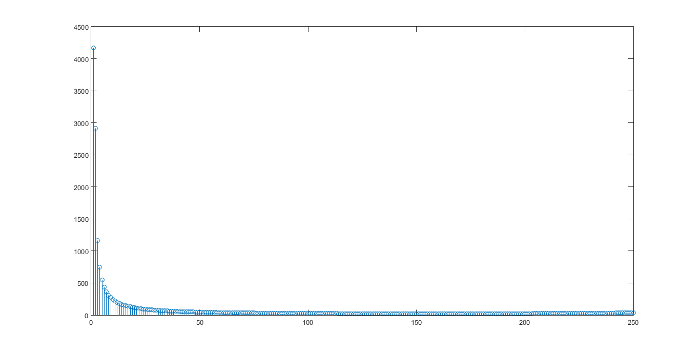
\includegraphics{stem2.png}
\end{center}

\subsection*{Gain versus }
\begin{center}
    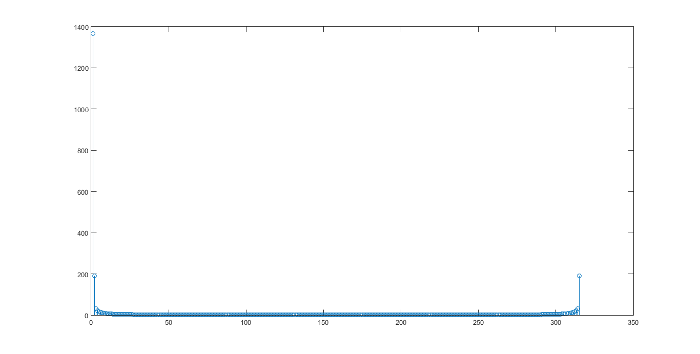
\includegraphics{stem3.png}
\end{center}


\section*{Results}

The bias point selected are as follows:

\begin{itemize}
\item i. Vm = 3.726 V

\item ii. Vm = 3.120 V

\item iii. Vm = 2.717 V
\end{itemize}

From the plots, we infer that Vm value decreases and slop increases from case (i) to case (iii).This is the direct consequence of the formula Vout=VDD – KnRD(Vin-Vtn). It is apparent that if either KN or RD increase, slope increases and Vm decreases.


\subsection*{SMALL SIGNAL OUTPUT CHARACTERISTICS (CALCULATION OF THD)}

Now, we shift our origin to (Vm,VDD/2) and clip out the cut-off and triode parts and take only the region where the output is more or less linear. Following this, we use a degree 3 polynomial to fit the data (using inbuilt function polyfit), give a sinusoidal input array (Sin(ώt)) and then take the fast-Fourier transform (using inbuilt function fft) of the obtained output to study the non-linearity of the amplifier. Following are the amplitude spectrum plots obtained:The given plots are for Case 1, Case 2 and Case 3 respectively.

Now, let us calculate the values of Total Harmonic Distortion for the three
different gain values (the three different cases)
\begin{center}
 \begin{tabular}{|| c | c| c ||}
 \hline
 \hline
 THD$_1$ & THD$_2$ & THD$_3$ \\
 \hline\hline\\
 -9.59 & 0.104 & 0.72\\
 \hline
\end{tabular}
\end{center}
 
\subsection*{ ADDITIONAL LINEARITY TESTS }

We calculate the Total Harmonic Distortion (THD) by taking inputs of different peak to peak values.
THD1(for amplitude 0.5 Vp-p) = 8.58\%
THD1(for amplitude 1.0 Vp-p) = 11.26\%
THD1(for amplitude 2.0 Vp-p) = 21.42\%

We can see that as input signal amplitude is increased, the total harmonic distortion increases. It is obvious because the input signal is affected by non-linear gain area due to change in curvature of fitted curve (In this case we used 6th
degree polynomial) and hence gets distorted.Now, we check the degradation of THD as the bias point is skewed away from (Vm,VDD/2). It is expected that closer the bias point is to VDD/2 the lesser the THD, since the entire input signal we lie in the linear range.

We perform this check for again the first set of data. We take the bias point as 4.16V skewing away from 3.727V.

THD1 = 17.01\%
(skewed case)

Next we try to see the THD values when we cascade amplifiers of different gains. Then we try to observe the difference between the cases when low gain amplifier is kept at first stage versus when high gain amplifier is kept at second stage. Following are the amplitude spectrum plots for the two cases:

THD$_1_-_>_2$(low->high gain) = 23.27\% 
THD$_2_-_>_1$(high->low gain) = 7.87\%

So, we see that when the high gain amplifier is taken as the first stage, we get a lesser value of THD. It is because the output of the first amplifier (high gain) is fed into the low gain amplifier. There is a fair chance that the signal may enter the non-linear region. But due to low gain the effect of non-linearity is quite suppressed as compared to the other case.

\section*{Discussion}

\subsection*{14EC10043}
From the characteristics we could observe that in the output characteristics as Vds increases the Id increases upto the transition point.

After the transition the curve didn’t remain perfectly horizontal as expected and this due to the channel width modulation effect.

While measuring Id with respect to Vgs we must keep Vds constant in our experiment we must adjust the value of drain resistance to keep Vds constant it was found roughly constant

\subsection*{14EC10049}
 
\begin{itemize}
\item When giving the input signal, it is important to ensure that the input span iswithin the linear region. For this purpose, input had to be scaled, especially when the gain is very high, as in the case of cascade amplifier configuration. For cascade amplifier, we have used input voltage of 0.1Vp-p.

\item For completely linear output, THD=0\% and the amplifier is said to be a linear amplifier.

\item As bias point is skewed away from (Vm,VDD/2), the new dc biasing is closer to the non-linear region and the same Vp-p causes more distortion. As a result, the THD obtained is higher.

\item We get a higher value of THD for higher value of gain. This depicts the gain-linearity tradeoff.

\item It is important to note that we do not consider the dc component of output signal while calculating the THD, as it is only because of the harmonics of the fundamental frequency.

\item To find Vm, rather than using the discrete derivative curve or it’s smoothened counterpart (using moving average smoothing), we prefer taking the derivative of a Fourier or Gaussian fit as it is more exact and gives us a more accurate value of Vm. In our case we went on with Gaussian fit because it was observed to be more accurate of the two. It is worth noting that for the optimum performance of these fitting techniques the input needs to be equi-spaced or they tend to diverge at places where concentration of input is low.




\end{document}


















